\chapter{Sizing of Hardware}
\label{chap:sizing}
This chapter details the sizing of the various components of the design chosen in Chapter \ref{chap:mech_design}.
The major parts of this process are,
\begin{enumerate}
\item
Masses of the platform and the leg
\item
Dimensions of the reaction wheel based on the above masses
\item
Choice of winding and reaction wheel motors
\end{enumerate}

\section{$2$ mass problem}
\begin{figure}[!h]
\centering
\begin{tikzpicture}[scale=0.45]
\draw (-3,0) -- (3,0);
\foreach \x in {-2.5,-2,...,2.5}
\draw (\x,0) -- (\x+0.5,-0.5);

\path (-2,7) coordinate(M1);
\path (2,10) coordinate(M2);
\path (-0.6,2) coordinate(m1);
\path (0.6,3.2) coordinate(m2);

\draw [thick](M1) rectangle (M2) node[midway]{\huge{$M$}};
\draw [thick](m1) rectangle (m2) node[midway]{\Large{$m$}};

\path (-2.5,0) coordinate (O);
\path (-2.5,2.6) coordinate (SPL);
\path (-2.5,8.5) coordinate (H);

\draw[<->] [semithick](O)++(-0.5,0) -- (-3,8.5) node[midway, left]{$H$};
\draw[<->] [semithick](SPL) -- (H) node[midway, right]{$l_0$};


\draw[snake=coil, segment amplitude=8pt] (0,3.2) -- (0,7) node[midway,right=2ex]{$k$};
\end{tikzpicture}
\caption{2 mass problem}
\label{fig:4_2mass}
\end{figure}
The basic idea behind a hopper is like that of the 2 masses connected by a spring problem. If the system shown in Fig.
\ref{fig:4_2mass} is allowed to fall from a height, the heavier mass pulls the smaller mass with it back into the air
after impact. Every cycle is accompanied by a loss in energy due to the inelastic impact of the smaller mass with the
ground. If we pump this energy back into the system using an external agent in every cycle, we can ensure sustained
hopping at the chosen height. The 2 mass problem can thus be taken as a basis to compute the range of values of masses
for acceptable performance. The following assumptions have been used in the simulation that follows,
\begin{enumerate}
\item
Dropping height (H) : 0.6 m
\item
Spring constant (k) : 300 N/m
\item
Spring relaxed length ($l_0$) : 0.3 m
\item
Trapezoidal profile for $\omega$ of the winding motor (constant $\alpha$ at the start and end)
\item
Faulhabeur 2342CR024 motor with a 3.71 reduction gear-box for comparison of torques
\item
Neglect energy loss due to friction
\end{enumerate}
It is seen from Fig. \ref{fig:4_2mass} that if $h_i$ are progressive heights, we have the relation,
\begin{equation}
h_n = \frac{Mh_{n-1} + ml_0}{M + m}
\end{equation}
\begin{equation}
\label{eqn:4_eloss}
E_{loss} = \frac{Mg\;(H-l_0)}{1 + M/m}
\end{equation}

\begin{figure}[!h]
\centering
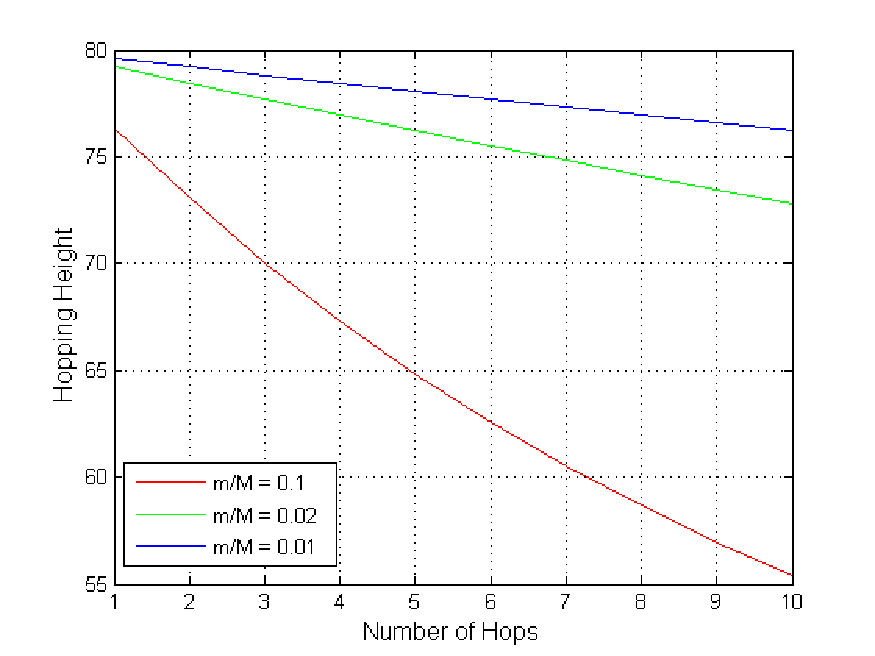
\includegraphics[scale=0.8]{fig/2mass_hopheight.pdf}
\caption{Hopping height for different M/m}
\label{fig:4_hopping_height}
\end{figure}
From Fig. \ref{fig:4_hopping_height}, it is seen that larger the ratio M/m, i.e. smaller the leg
mass, less is the loss in energy resulting in more number of hops. This is also seen for a increasing M. We would however,
like the M to be within limit too as we will also need to pump in extra energy into the system if the desired hopping
height is more than the starting height.
\begin{figure}[!h]
\centering
%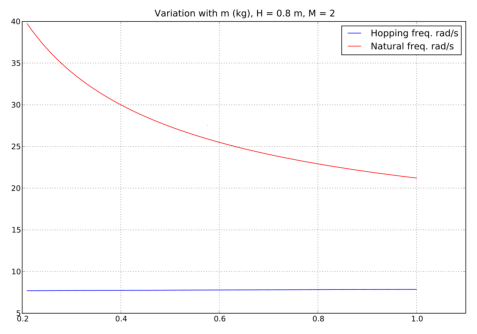
\includegraphics[scale=1.5]{fig/freq_m.pdf}
\caption{Torque variation with m}
\label{fig:4_torque2mss}
\end{figure}

\textbf{Change simulation to take care of torque for a rack and pinion}

\section{Impact analysis}
\label{sec:4_impact}
The desired hopping height dictates a hopping frequency. Smaller hopping height results in large number of impacts per time
and consequently in larger energy loss per unit time. However, beyond this consideration, since the hopper is a spring mass
system, it possesses a natural frequency of its own. If the hopping frequency is near to this natural frequency, a large
amount of energy is taken away by impact forces in every cycle. We intend to arrive at a range of values for the masses
to ensure a large difference between the hopping frequency ($\omega_{hop}$) and the natural frequency ($\omega_{nat}$).
The details of this analysis are as follows,
\begin{itemize}
\item 
Conserve energy at H and the moment of maximum extension of the spring after $t_{touchdown}$ to get the minimum height of the
fully extended platform above the leg. This comes out to be 8 cms for m = 0.4 kg. This value also reduces with increasing m. I
assumed no pre-extension of the spring while calculating this. The final value will be less then 8 cms if we take it into account.
Thus we say that the leg should protrude about 12 cms beyond the maximum extension of the platform which is obtained from Fig.
\ref{fig:4_hopping_height}.
\item
If $x_2$ is the height of C.G. just before touchdown, we can calculate the time taken for it to fall from a height H to $x_2$ as
$t_1$.
\item
M undergos simple harmonic motion from time $t_1$ till liftoff, and this time of motion is $t_2$
\item
M transfers its momentum at $t_1 + t_2$ to m resulting in a velocity $v_{cg, t_{2}}$ for the C.G. To ensure that M has largest
velocity while transfering momentum to m, we need to put a mechanical stopper at the natural length of the spring.
\item
The resultant velocity is just enough for the C.G. to reach a height H in time $t_3$.
\item
Total hopping time T = $t_1 + t_2 + t_3$, with $\omega_{hop} = \frac{2\pi}{T}$.
\item
$\omega_{nat} = \sqrt{\frac{k\;(1+m/M)}{m}}$
\end{itemize}

\begin{figure}[!h]
\centering
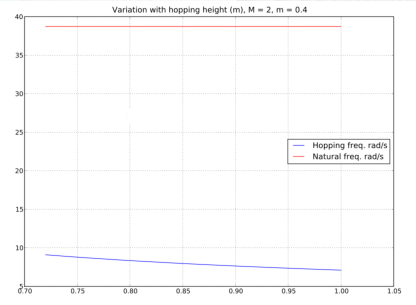
\includegraphics[scale=1.5]{fig/freq_hopheight.pdf}
\caption{Frequency variation with hopping height for M/m = 5}
\label{fig:4_freq_height}
\end{figure}
Fig. \ref{fig:4_freq_height} shows that $\omega_{hop}$ and $\omega_{nat}$ are seperated by large gap for the usable range
of values of hopping height. A similar analysis for variation of M also reveals that the two frequencies are seperated
by a large gap for all usuable values.
\begin{figure}[!h]
\centering
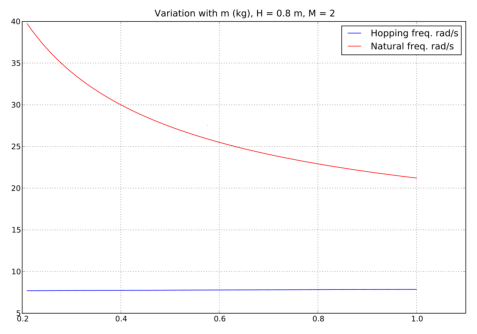
\includegraphics[scale=1.5]{fig/freq_m.pdf}
\caption{Frequency variation with m}
\label{fig:4_freq_m}
\end{figure}
Fig. \ref{fig:4_freq_m} succintly depicts all the above analysis. As the leg mass increases, the hopping frequency goes
closer to the natural frequency i.e. more impact per unit time. To compound matters, more and more energy is lost per impact
as per Eqn. \ref{eqn:4_eloss}. So the conclusion from impact analysis is that the leg mass should be as low as possible. It is also
seen from Fig. \ref{fig:4_freq_m} that \mbox{m = 0.4 -- 0.6 kg} is a good solution as well as an achievable one. 

\section{Reaction wheel}
For achieving a running gait with the hopper, it has to be started with the exact initial pitch and horizantal velocity.
For any other initial condition, the hopper is pitch unstable and will not be able to continue the running gait.
As mentioned in (cite shanmukh...), an offset mass acts as a passive stabilization to the pitch attitude of the hopper.
To get rid of this need for exact initial condition which is quite impractical, we design a reaction wheel on the hopper.
This will result in torque coupling on the pitch axis and thus provide an active control over the pitch of the robot.
The coupling equation can be written as,
\begin{equation}
J_{wheel}\;\omega_{wheel} = -(J_{wheel} + J_{body})\;\omega_{body}
\end{equation}
\begin{figure}[!h]
\centering
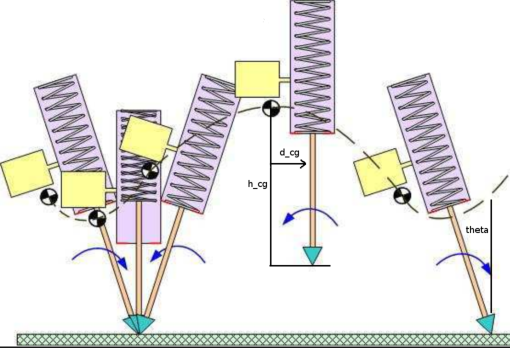
\includegraphics[scale=1.2]{fig/slom_motion.pdf}
\caption{Stabilizing impact torque due to SLOM}
\label{fig:4_rewac}
\end{figure}
The following considerations are made for this analysis,
\begin{itemize}
\item
The reaction wheel is taken as a ring with mass concentrated at the rim.
\item
Let $\theta_{impact}$ be the impact pitch attitude and $\theta_{liftoff}$ be the lift-off attitude. Pitch is measured with respect to
the vertical direction. An upright hopper means a pitch of zero.
\item
From Fig. \ref{fig:4_rewac}, the stabilizing impact torque is given by $\tau_{impact} = m\:v_{impact}\:(h_{cg} sin\:\theta + d_{cg}
cos\:\theta)$. This is positive torque and generates a pitch up. Thus we have a $\omega_{liftoff} = \tau_{impact}\:/J_{body}$
\item
The angle rotated due to horizantal velocity in the stance phase is $\Delta\:\theta = -v_h\:/h_{cg}\:\Delta\:t$. This means
$\theta_{liftoff} = \theta_{impact} + \Delta\:\theta$.
\item
The lift-off pitch needs to be corrected to $\theta_{impact}$ while the hopper is in the air. $\omega_{liftoff}$ might not be enough
to correct this pitch and so we need an additional reaction wheel.
\item
We assume a trapezoidal profile for $\omega_{wheel}$ with length of the plateau taken as $0.3\:T_{air}$. The acceleration phase is
$0.2\:T_{air}$ on either side. This means that we finish the reorientation task within 7/10 ths of the total time the hopper remains in
the air ($T_{air} = t_1 + t_3$ from Section \ref{sec:4_impact}).
\end{itemize}
\begin{figure}[!h]
\centering
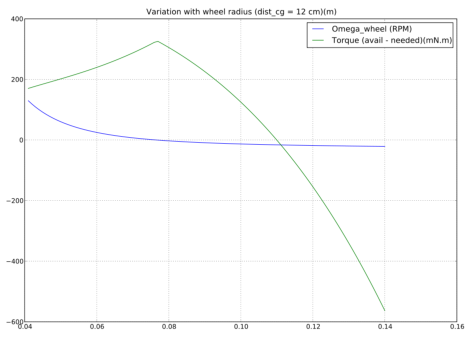
\includegraphics[scale=1.8]{fig/rewac_radius.pdf}
\caption{Torque requirements vs wheel radius}
\label{fig:4_rewac_radius}
\end{figure}
\begin{figure}[!h]
\centering
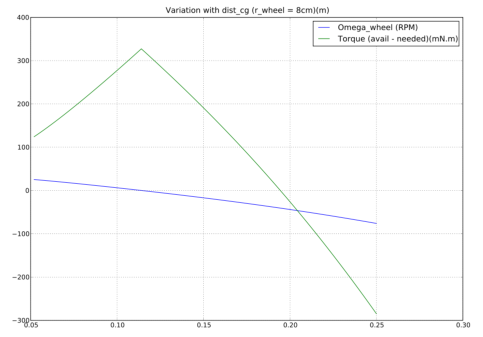
\includegraphics[scale=1.8]{fig/rewac_dist.pdf}
\caption{Torque requirements vs C.G. offset}
\label{fig:4_rewac_dist}
\end{figure}

\subsection{Results}
It is seen from Figs. \ref{fig:4_rewac_radius} and \ref{fig:4_rewac_dist} that a reaction wheel radius of 8 cm with a C.G. offset
of 12 cms lie near the peak of both the plots. They can be taken as the final values for fabricating the hopper.

\section{Choosing the Motors}






